\documentclass[supercite]{HustGraduPaper}
%进行个人信息设置
\title{RIS辅助的无线通信系统的原型验证} %论文题目
\author{裴熙隆} %作者姓名
\date{\today} %日期,默认当日
\school{人工智能与自动化学院} %院系名称
\classnum{自动化1705班} %专业班级
\stunum {U201714286} %学号
\instructor{陈忠、尹海帆} %指导教师姓名

%添加自己要用的其他宏包
\usepackage{xltxtra}
\usepackage{bm}
\usepackage{array}
\usepackage{multirow}
\usepackage[caption=false,font=footnotesize]{subfig}
\usepackage{algorithm}
\usepackage{algorithmic}

\begin{document}
	%生成标题页 \maketitle[可选参数]\end{document}\end{document}
	%可选参数:
	%logo color=green/black 华中科技大学字样的颜色,绿色或者黑色,默认绿色
	%line length=12em 填写信息处横线的长度,默认12em
	%line font=huawenzhongsong 填写信息的字体,默认huawenzhongsong
	\maketitle
	
	%生成声明与授权书页 \statement[可选参数]
	%可选参数:
	%confidentiality=yes/no/true/false/empty
	%是否保密,yes/true为保密;no/false为不保密,empty为不填,默认为empty
	%year=5 保密年数,默认为空
	\statement[confidentiality = false]
	
	\clearpage %结束上一页
	\pagenumbering{Roman} %摘要页码为大写罗马数字
	
	%填写中文摘要内容和关键字
	\begin{cnabstract}{可重构智能表面;智能反射面;RIS;IRS;LIS;超表面;超材料;无线中继;MIMO;大规模MIMO;原型系统;现场试验}
		%请注意使用中文分号“;”分割关键词!
		
		近年来
		
	\end{cnabstract}
	%填写英文摘要内容和关键字
	\begin{enabstract}{Reconfigurable intelligent surface; intelligent reflecting surface; RIS; IRS; LIS; metasurface; metamaterial; wireless repeating; MIMO; massive MIMO; prototype; field trials}
		%Please Use English Semicolon and a Space "; " to Separate  Keys! 

		Recently, 

	\end{enabstract}
	
	%生成目录 \tableofcontents[可选参数]
	%可选参数:
	%pagenum=yes/no/true/false 目录是否显示页码,默认为false
	%toc in toc=yes/no/true/false 目录中是否有目录及其页码,默认为false
	%level=4 目录级数,默认是4,即显示到subsubsubsection
	%section indent=0em 目录第一级的缩进,默认是0em
	%subsection indent=1.5em 目录第二级的缩进,默认是1.5em
	%subsubsection indent=3.8em 目录第三级的缩进,默认是3.8em
	%subsubsubsection indent=7em 目录第四级的缩进,默认是7em
	%paragraph indent=11em 目录第五级的缩进,默认是11em
	%subparagraph indent=13em 目录第六级的缩进,默认13em
	%indent=normal/noindent/hustnoindent/sameforsubandsubsub 快速缩进设置,具体见文档
	%dot sep=4.5 目录点间距,默认4.5
	%section dot sep=4.5 目录第一级的点间距,默认是4.5
	%subsection dot sep=4.5 目录第二级的点间距,默认是4.5
	%subsubsection dot sep=4.5 目录第三级的点间距,默认是4.5
	%subsubsubsection dot sep=4.5 目录第四级的点间距,默认是4.5
	%paragraph dot sep=4.5 目录第五级的点间距,默认是4.5
	%subparagraph dot sep=4.6 目录第六级的点间距,默认是4.5
	%请注意在合适的位置放置\pagenumbering{numstyle}使用新的页码
	\tableofcontents
	
	\clearpage%结束上一页
	\pagenumbering{arabic} %正文页码为阿拉伯数字
	
	%正文内容从这里开始
	\section{绪论}
	%这是小四号的正文字体,段间距1.5倍
	%通过空一行实现段落换行,仅仅是回车并不会产生新的段落
	%\par 也可以通过\verb|\par|命令来新起一段
	
	\subsection{课题背景及意义}
	
	这个课题有什么意义呢

	\subsection{国内外现状分析}
	
	\section{相关理论}
	
	啊这,不知道有什么原理呢。
	
	\section{系统设计}	
	
	这个系统怎么设计呢?\footnote{哈哈哈}
	
	\section{实验数据}

	\section{段落}
	\paragraph{段落}\label{para:para}这是一个带有顶头标签的段落这是一个带有顶头标签的段落这是一个带有顶头标签的段落这是一个带有顶头标签的段落这是一个带有顶头标签的段落这是一个带有顶头标签的段落这是一个带有顶头标签的段落
	\subparagraph{小段落}\label{subpara:subpara}只是一个带有缩进标签的段落只是一个带有缩进标签的段落只是一个带有缩进标签的段落只是一个带有缩进标签的段落只是一个带有缩进标签的段落只是一个带有缩进标签的段落只是一个带有缩进标签的段落
	\subsection{第二小节}
	本模板已经引入伪加粗和伪斜体,这样就不需要对应的粗体和斜体字体也能生成需要的效果,就像下面这样
	
	{\songti \bfseries 宋体加粗}
	
	{\songti \itshape 宋体斜体}
	
	{\songti \bfseries \itshape 宋体粗斜体}
	
	请注意,使用加粗和斜体时,请与字体名称一同使用,否则会自动将粗体匹配为黑体,斜体匹配为楷体,就像下面这样
	
	{正常显示宋体}
	
	{\bfseries 加粗后变为黑体}
	
	{\itshape 斜体后变为楷体}
	
	\subsection{第三小节}
	
	
	上市
	en 
	\begin{algorithm}
		\caption{Greedy Fast Beamforming Algorithm}
		\label{alg:GreedyAlgorithm}
		\begin{algorithmic}[1]
			\STATE \textbf{Input: } The feedback of RX signal power $p_t$.
			\STATE \textbf{Output: } The reflection coefficients matrix.
			\STATE Initialize a reflection coefficients matrix $ \mathbf{R}_0\in \mathbb{C}^{M \times N }$;
			\STATE Receive initial feedback of the RX signal power $ p_0 $;
			
			\STATE // Horizontal search;
			\FOR {each $n \in [1, N]$}
			\STATE  $ \mathbf{R}_{n} \leftarrow [\mathbf{r}_{n-1,1},\cdots,\mathbf{r}_{n-1,n-1},- \mathbf{r}_{n-1,n}, \mathbf{r}_{n-1,n+1}\cdots,\mathbf{r}_{n-1,N}] $;
			\STATE Receive feedback $ p_{n} $ using configuration $ \mathbf{R}_{n}$;
			\IF {$ p_{n-1} \ge p_{n}$}
			\STATE $ \mathbf{R}_{n} \leftarrow \mathbf{R}_{n-1}$;
			\ENDIF
			\ENDFOR
			\RETURN{reflection coefficients matrix $ \mathbf{R}_{N}$;}
			
			\STATE // Vertical search;
			\STATE Denote $ \mathbf{R}_{N} =[\mathbf{s}_{N,1},\mathbf{s}_{N,2},\cdots,\mathbf{s}_{N,M}]^\mathrm{T}$;
			\FOR {each $m \in [1, M]$}
			\small
			\STATE  $\mathbf{R}_{N+m} \leftarrow [\mathbf{s}_{N+m-1,1},\cdots,\mathbf{s}_{N+m-1,m-1},- \mathbf{s}_{N+m-1,m}, \mathbf{s}_{N+m-1,m+1}, \cdots, \mathbf{s}_{N+m-1,M}]^\mathrm{T}$;
			\normalsize
			\STATE Receive feedback $ p_{N+m} $ using configuration $\mathbf{R}_{N+m}$;
			\IF {$ p_{N+m-1} \ge p_{N+m}$}
			\STATE $ \mathbf{R}_{N+m} \leftarrow \mathbf{R}_{N+m-1}$;
			\ENDIF
			\ENDFOR
			\RETURN{reflection coefficient matrix $ \mathbf{R}_{M+N}$.}
		\end{algorithmic}
	\end{algorithm}
	
	
	
	
	
	
	
	
	
	\section{参考文献和交叉引用}\label{sec:ref}
	\subsection{参考文献}
	这是一个参考文献引用的范例\cite{9326394, Renzo2019,5502350, liang2019large, CHN_zhou2020, CHN_zhang2017}
	

	
	
	\subsection{交叉引用}\label{subsec:crossref}
	本模板已经重写了hyperref宏包的\verb|\autoref|命令,方便引用章节、公式和图表。
	
	比如说\autoref{sec:ref}和\autoref{subsec:crossref}就引用了本章节,\autoref{para:para}和\autoref{subpara:subpara}引用了之前的两个段落。显然段落因为没有序号,引用结果和上一节的需要相同,因此建议使用段落“\nameref{para:para}”和段落“\nameref{subpara:subpara}”。
	
	\section{公式这么用}
	在文中引用公式可以这么写:$a^2+b^2=c^2$这是勾股定理,他还可以表示为$c=\sqrt{a^2+b^2}$,还可以让公式单独一段并且加上编号
	\begin{equation}
	\sin^2{\theta}+\cos^2{\theta}=1 \label{eq:pingfanghe}
	\end{equation}
	还可以通过添加标签在正文中引用公式,如式~\eqref{eq:pingfanghe}~或者\autoref{eq:pingfanghe}。我们还可以轻松打出一个矩阵
	\begin{equation}
	\bm{A}=\begin{bmatrix}
	1&2&3&4\\
	11&22&33&44\\
	\end{bmatrix}
	\times\begin{bmatrix}
	22&24\\
	32&34\\
	42&44\\
	52&54\\
	\end{bmatrix}
	\end{equation}
	或者多个带编号的公式
	\begin{eqnarray}
	f_1(x)=12x^2+36x+\sin x\\
	f_2(x)=\sqrt{3}{x^3+3x}
	\end{eqnarray}
	以上
	
	\section{用图和表的示例}
	\subsection{图的使用}
	\XeLaTeX 环境下可以使用EPS、PDF、PNG、JPEG、BMP格式的图片,当然也可以用绘图包直接在\LaTeX 中绘制图形,推荐使用宏包tikz。图的环境是figure,但figure环境使用复杂且不自带标题,因此本模板定义了一个通用版本的generalfig,该环境会将figure内的图片居中并设置标签与引用名,同时会让图片位置设置为所有可行位置(htbp,即此处、页顶、页底、独立一页),此选项可以作为可选参数设置。
	
	其使用方法如下:\autoref{fig:50mcopper}

	\autoref{fig:50mtest}

	\ref{fig:50mcopper}

	\ref{fig:50mtest}
	
	\begin{figure}[t!]
		\centering
		\subfloat[df哈哈]{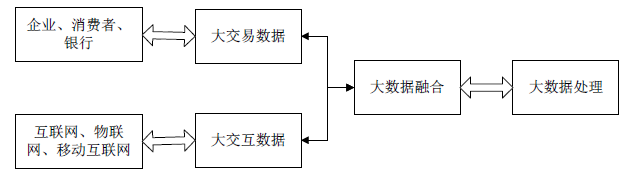
\includegraphics[width=0.5\linewidth]{Figures/data.png}%
			\label{fig:50mphoto}}
		\hfil
		\subfloat[dd]{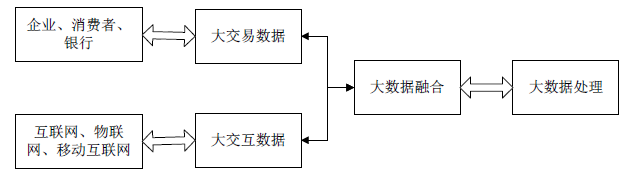
\includegraphics[width=0.5\linewidth]{Figures/data.png}%
			\label{fig:copper}}
		\hfil
		\subfloat[fs]{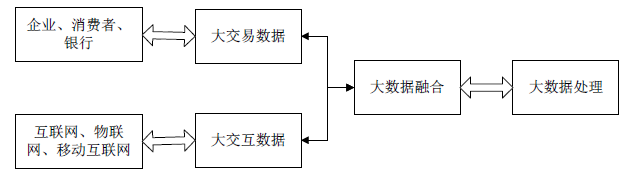
\includegraphics[width=0.5\linewidth]{Figures/data.png}%
			\label{fig:50mgreedy}}
		\hfil
		\subfloat[dfdf]{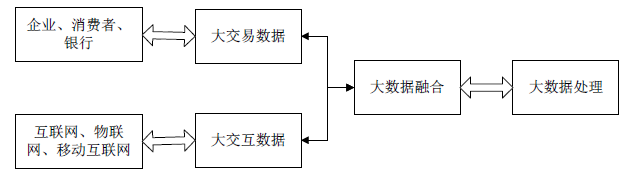
\includegraphics[width=0.5\linewidth]{Figures/data.png}%
			\label{fig:50mcopper}}
		\caption{The 50 m outdoor over-the-air test: (a) the scene of the transmitter and receiver; (b) a copper plate of the same size as the RIS; (c) spectrum when using the RIS; (d) spectrum when using the copper plate.}
		\label{fig:50mtest}
	\end{figure}

	\begin{figure}[htb]
		\centering
		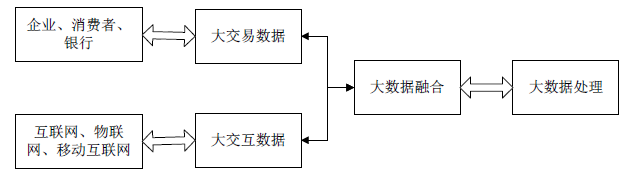
\includegraphics[width=0.5\linewidth]{Figures/data.png}
		\caption{Indoor non-LoS test.}
		\label{fig:through_wall}
	\end{figure}

	\begin{generalfig}[htb]{大数据信息处理框架}{fig:data}
		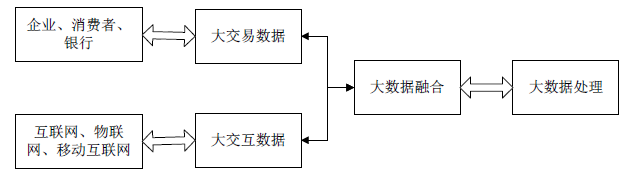
\includegraphics[width=0.4\linewidth]{Figures/data.png}
	\end{generalfig}
	
	同时也可以引用该图片例如:\autoref{fig:data}或者图~\ref{fig:data}。请注意generalfig第一个参数是标题,第二个参数是引用。
	
	\newpage
	
	\subsection{表的使用}
	作为论文,推荐使用三线表进行排版。所谓三线表,即在标题前有横线,标题后有横线,表格最后还有横线,其他地方无线。当然这不是死规定,也可以根据需要在合适的地方加线。
	、踩踩踩
	本文定义了新的可变长度左中右(LCR)格式,LCR三个格式会根据表格宽度的设定自行控制宽度,且其宽度相等,方便设置和页面相同宽度的表格。但该功能需要使用tabularx做表。
	\begin{generaltab}{某校学生升高体重样本}{tab:heightweight}
		\begin{tabularx}{\textwidth}{lCCC}
			\toprule
			序号                              & 年龄 &   身高   &  体重   \\ \midrule
			1                               & 14 &  156   &  42   \\
			2                               & 16 &  158   &  45   \\
			3                               & 14 &  162   &  48   \\
			4                               & 15 &  163   &  50   \\
			\cmidrule{2-4} %添加2-4列的中线
			平均 & 15 & 159.75 & 46.25 \\ \bottomrule
		\end{tabularx}
	\end{generaltab}
	
	当然你也可以引用表格,就像这样:\autoref{tab:heightweight}。
	
	\section{列表的使用}
	这是一个计数的列表
	\begin{enumerate}
		\item 第一项
		\begin{enumerate}
			\item 第一项中的第一项
			\item 第一项中的第二项
		\end{enumerate}
		\item 第二项
		\item 第三项
	\end{enumerate}
	
	这是一个不计数的列表
	\begin{itemize}
		\item 第一项
		\begin{itemize}
			\item 第一项中的第一项
			\item 第一项中的第二项
		\end{itemize}
		\item 第二项
		\item 第三项
	\end{itemize}
	
	\begin{thankpage}
		感谢老师
	\end{thankpage}
	
	%生成参考文献
	%使用方法:\bibliography{参考文件1文件名, 参考文献2文件名, ...}
	\bibliography{Bibs/references_Gradu}
	
	\begin{appendices}
		\section{这是第一个附录}
		这里是附录环境,其中的section、subsection、subsubsection已经变为附录的样式,并且会以这种样式加入目录中。
		\subsection{附录可以有小节}
		\subsubsection{附录中也可以有小小节}\label{apxsubsubsec:appendix}
		\subsubsubsection{附录中也有小小小节}
		\verb|\autoref|无法识别Appendices环境,引用效果和正文一样,如\autoref{apxsubsubsec:appendix}。所以如果引用附录的话,建议直接使用附录~\ref{apxsubsubsec:appendix}。
	\end{appendices}
	
\end{document}




